\documentclass[ignorenonframetext]{beamer}

\mode<article>
{
  \usepackage{fullpage}
  \usepackage{pgf}
  \usepackage{hyperref}
  \usepackage{subfigure}
  \restylefloat{figure}
  \setjobnamebeamerversion{highorder.beamer}
}

\mode<presentation>
{
  \usetheme{Singapore}
  \usecolortheme{crane}	
  \setbeamercovered{transparent}
}
\date[19.04.2010]{April 19, 2010}

\usepackage[latin1]{inputenc}
\usepackage{listings}

\title{Parallel I/O using \texttt{MPI-IO}}
\author{Arne Morten~Kvarving}
\subject{Parallel programming, I/O}

\institute[IME]{
  Department of Mathematical Sciences\\
  Norwegian University of Science and Technology}

\newcommand{\ub}[1]{\underbar{$#1$}\,}

\begin{document}

\frame{\maketitle}
\frame[label=overview1]{
\frametitle{Why consider parallel I/O?}
	\begin{itemize}
		\item Supercomputers get faster and faster.
		\item This means the applications consume / produce more data.
		\item This can transform CPU bound problems to I/O bound problems.
		\item CPU processing is easily made massively parallel, I/O processing is harder.
	\end{itemize}
}
\frame[label=overview9]{
\frametitle{Available hardware}
	\begin{itemize}
		\item Secondary storage is typically hard disk drives.
			\begin{center}
				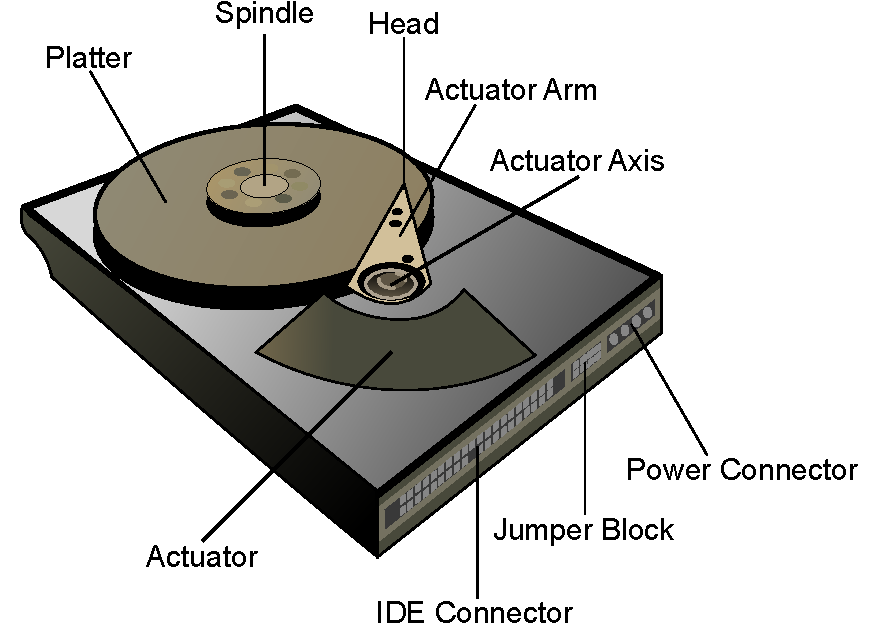
\includegraphics[width=8cm]{../../notes/09.mpi-io/Hard_drive-en}
			\end{center}
	\end{itemize}
}
\frame[label=read1]{
\frametitle{Reading data}
	\begin{itemize}
		\item Due to the serial nature of HDDs, even if several processes issue
			reads concurrently, they are performed in serial.
			\vspace{1cm}
		\begin{center}
			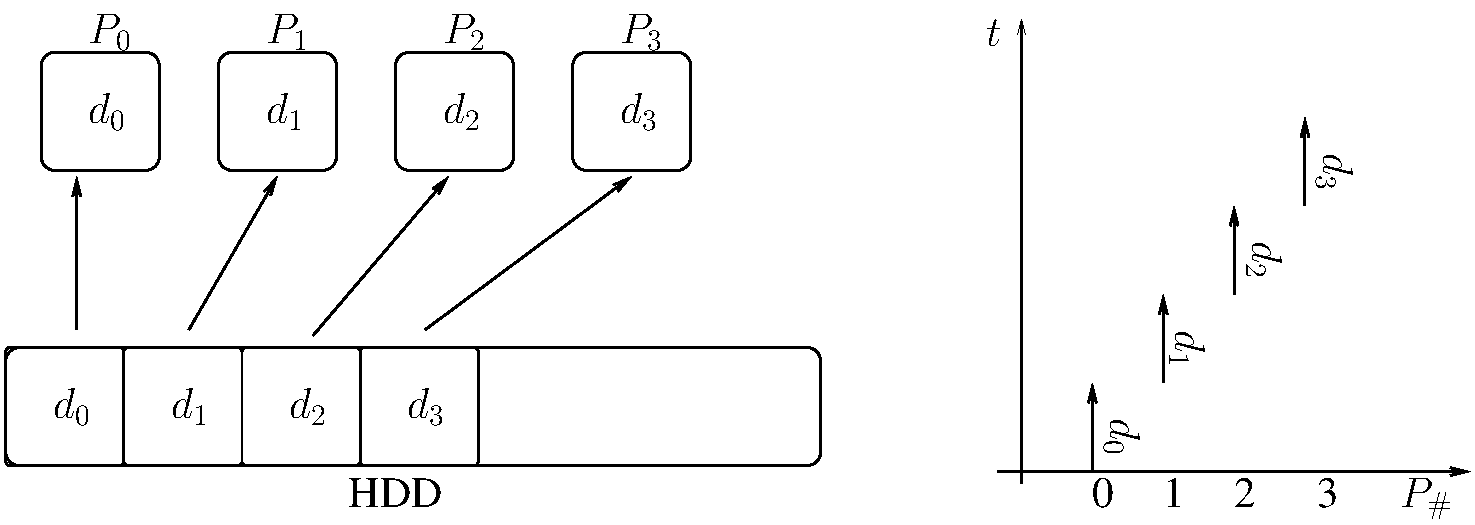
\includegraphics[width=8cm]{../../notes/09.mpi-io/many-onedisk}
		\end{center}
	\end{itemize}
}
\frame[label=read2]{
\frametitle{Reading data in parallel}
	\begin{itemize}
		\item This can be remedied by harnessing the aggregated bandwith of several devices.
		\vspace{1cm}
		\begin{center}
			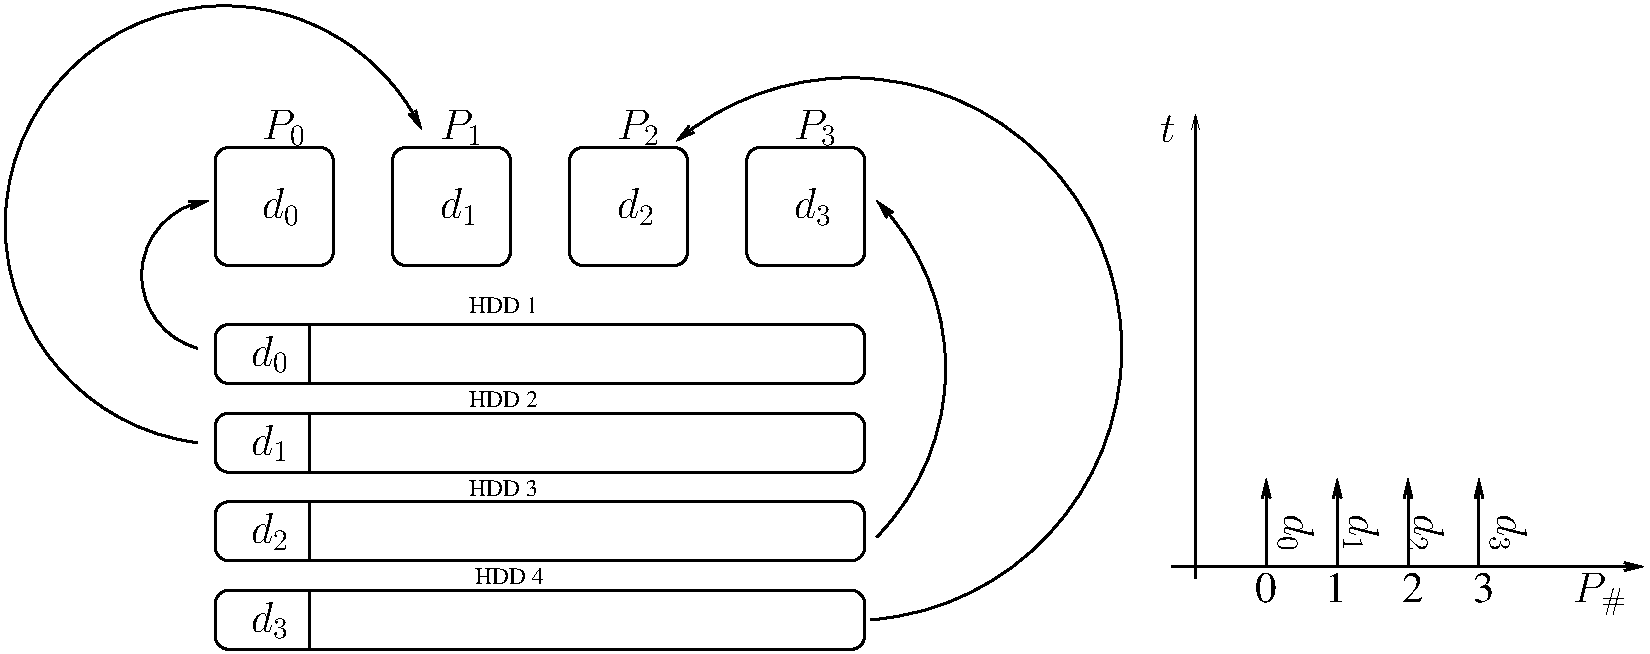
\includegraphics[width=8cm]{../../notes/09.mpi-io/many-manydisk}
		\end{center}
	\end{itemize}
}
\frame[label=write1]{
\frametitle{Writing data in parallel applications}
	\begin{itemize}
		\item Traditionally, HPC applications did the I/O in one of two ways;
			either \emph{post-mortem assembly} or serialization.
		\item In post-mortem assembly, each process dumps its data to a separate
			file, then a separate postprocessing application is written which
			stitches the data in a suitable format is written.
		\item This necessitates doing a lot more I/O than strictly required, and
			even if the data is initially written in parallel, the post-processing
			app will do it in a serial manner.
	\end{itemize}
}
\frame[label=write2]{
\frametitle{Writing data in parallel applications}
	\begin{itemize}
		\item In serialization the I/O is, as the name hints at, serialized.
			\begin{center}
				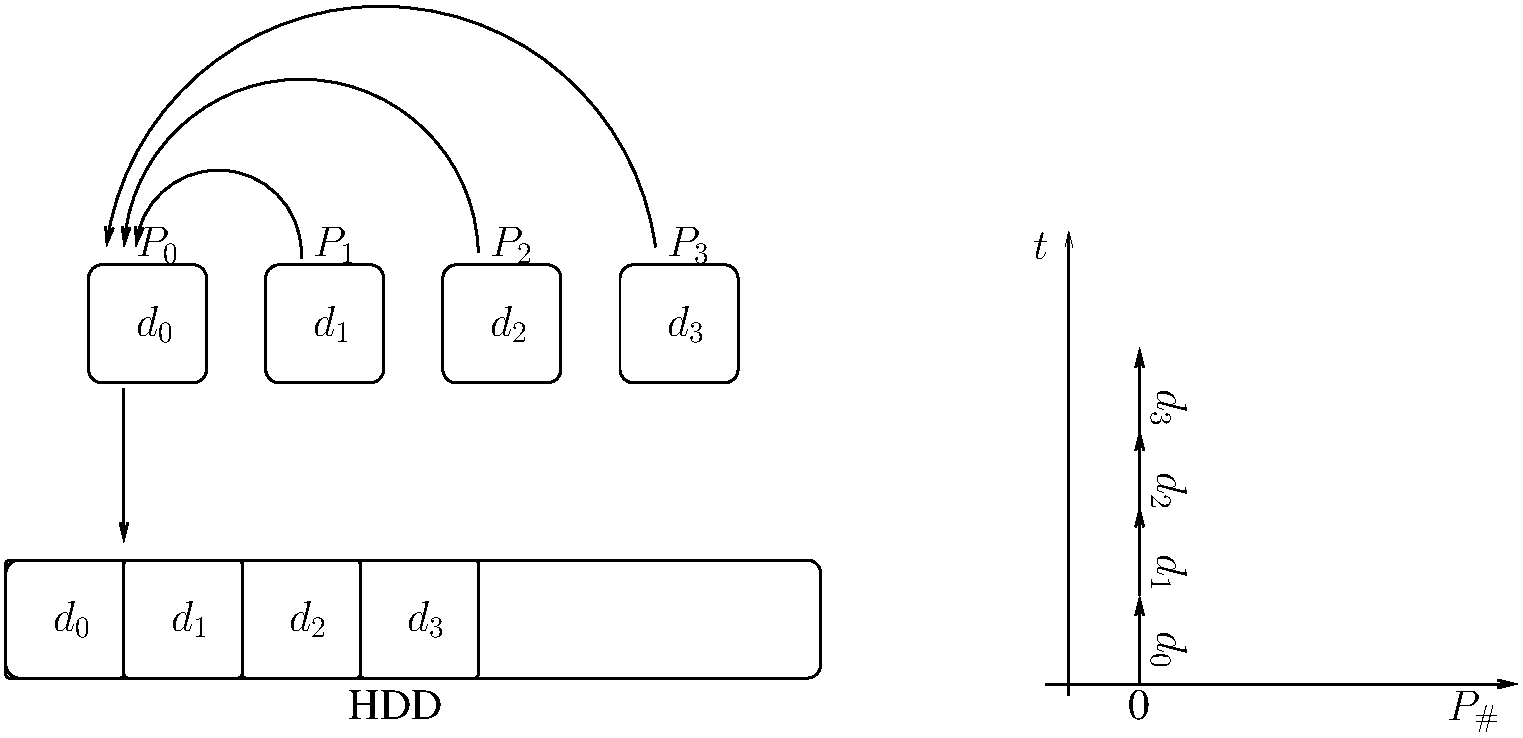
\includegraphics[width=8cm]{../../notes/09.mpi-io/serial}
			\end{center}
		\item Error prone since we often do not have the memory to store
			all data on a single node, which necessitates quite some data juggling.
	\end{itemize}
}
\frame[label=write3]{
\frametitle{Writing data in parallel applications}
	\begin{itemize}
		\item Thus we would like to be able to store all data in a single file
			spread across multiple physical storage devices, without having to
			fall back on serialization.
		\item \texttt{MPI-IO} allows us to do just this.
		\item Part of the \texttt{MPI} 2.0 standard.
		\item While \texttt{MPI-IO} is highly portable, tuning to the underlying
			filesystem is unavoidable to achieve high performance.
		\item On \texttt{NOTUR} machines, the \emph{general parallel filesystem}, GPFS, is
			used. We will not discuss any details here.
	\end{itemize}
}
\frame[label=mpiio1]{
\frametitle{\texttt{MPI-IO} - simple example}
	\begin{itemize}
		\item Assume we want to write data in the following pattern
			\begin{center}
				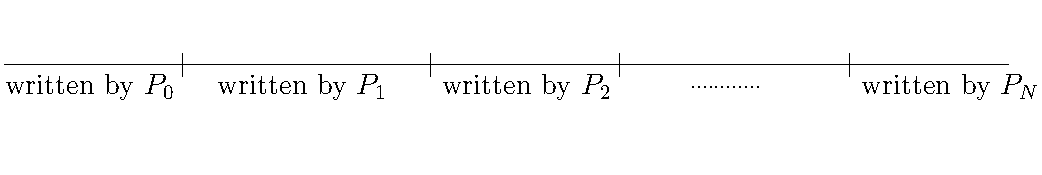
\includegraphics[width=8cm]{../../notes/09.mpi-io/slicedvector}
			\end{center}
		\item Such a data pattern would be present if we have partitioned a
			matrix in a strip pattern such as in the project task.
		\item If you are familiar with standard \texttt{POSIX} I/O, the following
			code should look quite familiar.
	\end{itemize}
}
\frame[label=mpiio2]{
\frametitle{\texttt{MPI-IO} - simple example}
	\begin{itemize}
		\item We start by opening a file handle.
			\lstinputlisting[language=C]{../../notes/09.mpi-io/open-handle.c}
	\end{itemize}
}
\frame[label=mpiio3]{
\frametitle{\texttt{MPI-IO} - simple example}
	\begin{itemize}
		\item There are basically two ways to write the data, both of which come in two flavours.
		\item Separate handles is perhaps the most natural. Exactly as in \texttt{POSIX}.
			\lstinputlisting[language=C]{../../notes/09.mpi-io/separate-handle-write.c}
	\end{itemize}
}
\frame[label=mpiio4]{
\frametitle{\texttt{MPI-IO} - simple example}
	\begin{itemize}
		\item Alternatively, we can use the \emph{explicit offset} version;
			\lstinputlisting[language=C]{../../notes/09.mpi-io/explicit-offset-write.c}
		\item Both of these using individual I/O calls on each process.
			An alternative is to use \emph{collective} calls.
	\end{itemize}
}
\frame[label=mpiio6]{
\frametitle{\texttt{MPI-IO} - simple example}
	\begin{itemize}
		\item The first one only differs by the write function.
			\lstinputlisting[language=C,basicstyle=\small]{../../notes/09.mpi-io/collective-write.c}
		\item The second uses shared file-pointers;
			\lstinputlisting[language=C,basicstyle=\small]{../../notes/09.mpi-io/shared-write.c}
		\item Finally we have to close the file handle;
			\lstinputlisting[language=C]{../../notes/09.mpi-io/close.c}
	\end{itemize}
}
\frame[label=mpiio7]{
\frametitle{Non-sequential I/O - fileviews}
	\begin{itemize}
		\item The simple data access/storage pattern we considered is
			only predominant in simple codes.
		\item Usually the access patterns in real code are much more involved.
		\item While programming such patterns naively using many seeks and
			many small writes are possible, it is nothing to be recommended.
		\item Highly error prone and bad for performance.
	\end{itemize}
}
\frame[label=mpiio8]{
\frametitle{Non-sequential I/O - fileviews}
	\begin{itemize}
		\item We now consider a vector split in a cyclic manner;
			\begin{center}
				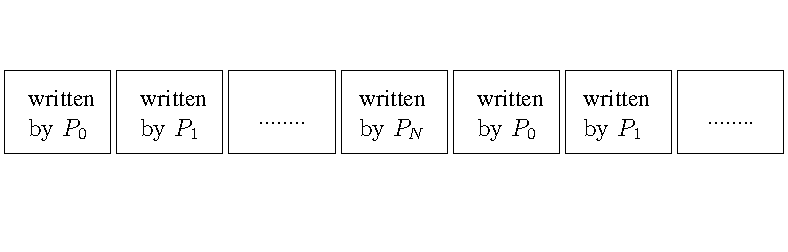
\includegraphics[width=8cm]{../../notes/09.mpi-io/splitvector}
			\end{center}
		\item Each block consists of a small amount of data.
		\item For simplicity, we here assume each block consists of a single 
			  double precision floating point number.
	\end{itemize}
}
\frame[label=mpiio9]{
\frametitle{Non-sequential I/O - fileviews}
	\begin{itemize}
		\item MPI has a builtin machinery to describe custom data types.
		\item These were originally intended to be used to describe data layout in memory.
		\item However, they can also be used to describe data patterns on secondary storage.
		\item From each separate process, the data access pattern consists of a single
			number followed by a gap of $size-1$ numbers.
	\end{itemize}
}
\frame[label=mpiio10]{
\frametitle{Non-sequential I/O - fileviews}
	\begin{itemize}
		\item We now construct this datatype;
			\lstinputlisting[language=C]{../../notes/09.mpi-io/createsplitview.c}
	\end{itemize}
}
\frame[label=mpiio11]{
\frametitle{Non-sequential I/O - fileviews}
	\begin{itemize}
		\item We then attach this datatype as a process' \emph{view} into the file using
			the function
			\[
				MPI\_File\_set\_view(fh,disp,datatype,viewtype,encoding,info)
			\]
		\item The specific code looks like
			\lstinputlisting[language=C]{../../notes/09.mpi-io/setsplitview.c}
		\item Notice the usage of the \emph{disp} field.
	\end{itemize}
}
\frame[label=mpiio12]{
\frametitle{Non-sequential I/O - fileviews}
	\begin{itemize}
		\item Writing the data to secondary storage is now just a normal
			write call on each process, i.e.,
			\lstinputlisting[language=C]{../../notes/09.mpi-io/writesplitview.c}
		\item The system takes care of inserting the gaps. Since it knows
			the data access patterns on each process up front, it can
			optimize how storing the data to disc is performed (large writes, no seeks).
	\end{itemize}
}
\frame[label=mpiio13]{
\frametitle{Non-sequential I/O - distributed arrays}
	\begin{itemize}
		\item In HPC applications, the data usually consists of matrices or 3D arrays.
		\item This fact has not gone past the \texttt{MPI} creators.
		\item \texttt{MPI} contains machinery to partition such arrays in semi-automatic ways.
		\item We now show that we also benefit from this when we want to write the data
			to secondary storage.
	\end{itemize}
}
\frame[label=mpiio14]{
\frametitle{Non-sequential I/O - distributed arrays}
	\begin{itemize}
		\item There are essentially two ways to split such an array across processes.
			\begin{center}
				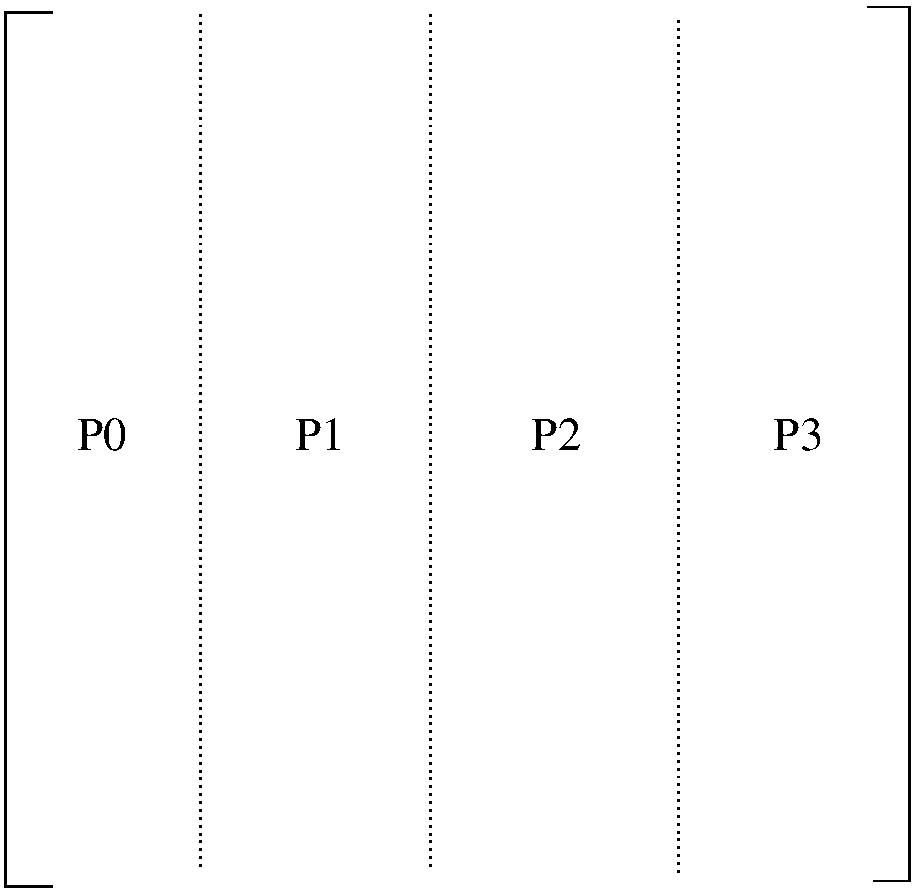
\includegraphics[width=4cm]{../../notes/09.mpi-io/strip}
				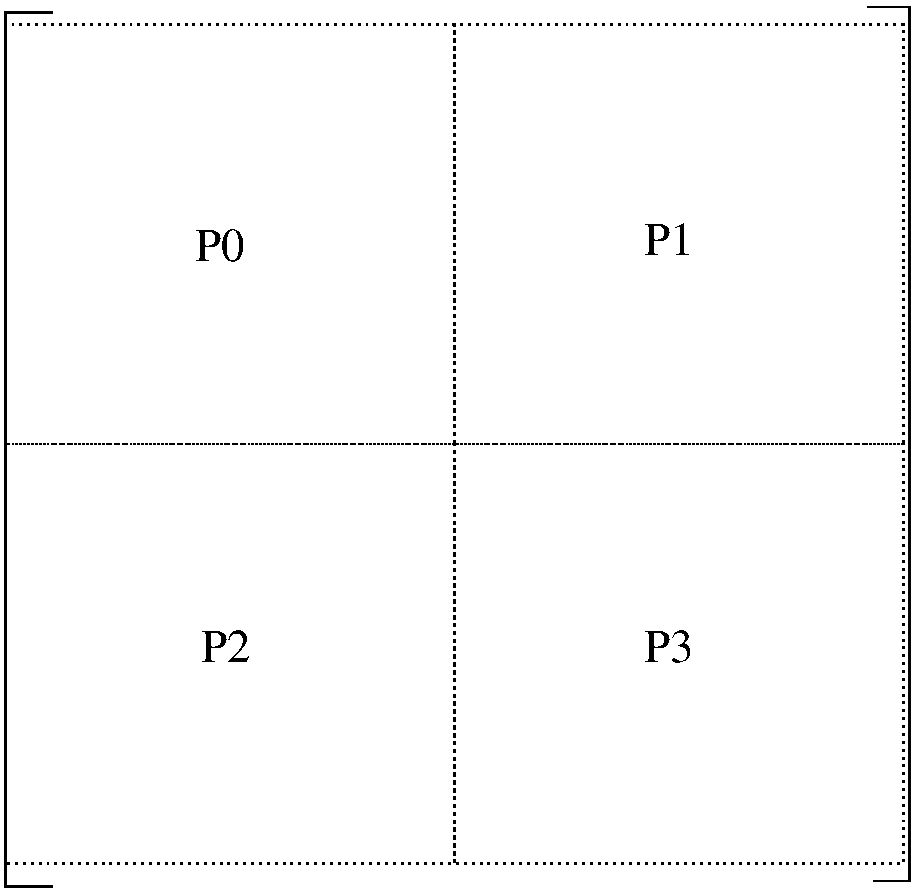
\includegraphics[width=4cm]{../../notes/09.mpi-io/block}
			\end{center}
		\item The \texttt{MPI} machinery allows us to handle both of these with essentially 
			the same code.
	\end{itemize}
}
\frame[label=mpiio15]{
\frametitle{Non-sequential I/O - distributed arrays}
	\begin{itemize}
		\item \texttt{MPI} names such arrays \emph{darrays} - distributed arrays.
		\item The available functions are heavily inspired by the \texttt{High Performance Fortran}
			standard.
		\item In the following we use the term \emph{topology}, which in layman's terms means
			``how stuff is connected''.
		\item An array partitioning consists of a topology and a mapping of processes onto this
			topology.
	\end{itemize}
}
\frame[label=mpiio16]{
\frametitle{Non-sequential I/O - distributed arrays}
	\begin{itemize}
		\item The following figure contains the pieces of information we need to describe the
			topology and the mapping.
			\begin{center}
				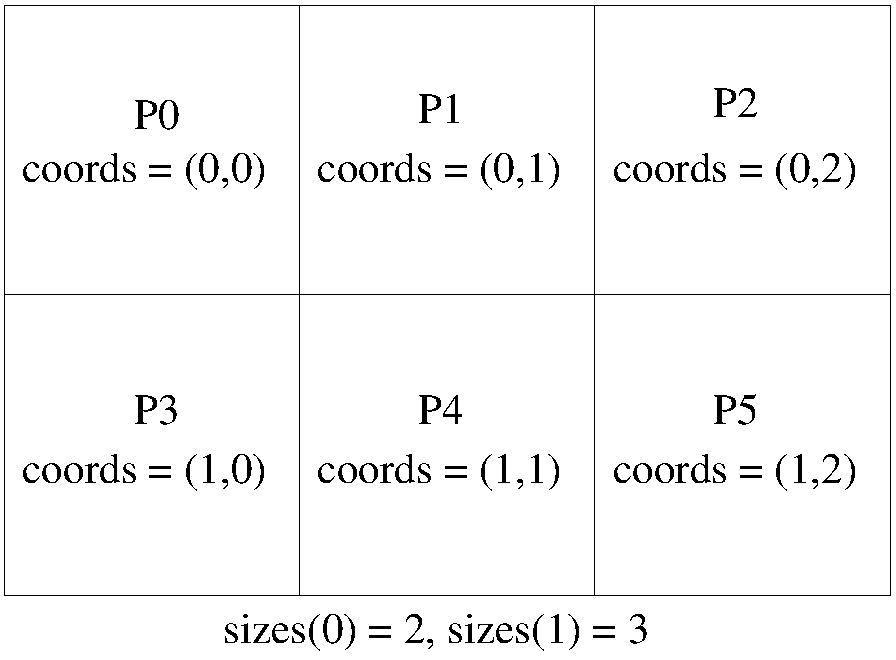
\includegraphics[width=8cm]{../../notes/09.mpi-io/splitdomain}
			\end{center}
	\end{itemize}
}
\frame[label=mpiio17]{
\frametitle{Non-sequential I/O - distributed arrays}
	\begin{itemize}
		\item A global topology - here a Cartesian topology expressed as the number 
			  of processes along each dimension (here 2 and 3, respectively).
		\item Location of a particular domain in the topology, again
			  this can be expressed as an integer along each dimension.
		\item A mapping of the available processes onto the topology.
	\end{itemize}
}
\frame[label=mpiio18]{
\frametitle{Non-sequential I/O - distributed arrays}
	\begin{itemize}
		\item The first function we use is \emph{MPI\_Dims\_Create}. This generates
			a Cartesian partioning.
		\item Block partioning: \lstinputlisting[language=C]{../../notes/09.mpi-io/dimsblock.c}
		\item Strip partioning: \lstinputlisting[language=C]{../../notes/09.mpi-io/dimsstrip.c}
		\item Upon return the \emph{dims} array holds the results.
	\end{itemize}
}
\frame[label=mpiio19]{
\frametitle{Non-sequential I/O - distributed arrays}
	\begin{itemize}
		\item In order to be able to generate the mapping of processes onto
			the topology, we need to define a communicator which has the
			topology attached.
			\lstinputlisting[language=C]{../../notes/09.mpi-io/comm.c}
		\item Upon return the \emph{comm} variable holds the new communicator.
	\end{itemize}
}
\frame[label=mpiio20]{
\frametitle{Non-sequential I/O - distributed arrays}
	\begin{itemize}
		\item The individual process can now query where they are placed in the
			topology using the function
			\lstinputlisting[language=C]{../../notes/09.mpi-io/coord.c}
		\item Upon return from the function, the \emph{coords} array holds the coordinates.
			For instance, it would hold 1 and 2 when called on process 5.
	\end{itemize}
}
\frame[label=mpiio21]{
\frametitle{Non-sequential I/O - distributed arrays}
	\begin{itemize}
		\item We can now use the function
			\[
				\begin{split}
					MPI\_Type\_create\_darray(size,rank,dims,gsizes, \\
											  distribs,dargs,sizes, \\
											  order,etype,newtype).
				\end{split}
			\]
			to generate the data type, and thus the file view, on each process.
		\item Non-obvious parameters; \emph{gsizes}, \emph{distribs}, \emph{dargs},
			\emph{order} and \emph{etype}.
	\end{itemize}
}
\frame[label=mpiio22]{
\frametitle{Non-sequential I/O - distributed arrays}
	\begin{itemize}
		\item \emph{gsizes} - global array dimensions.
		\item \emph{distribs} - distribution strategies along each dimension.
			Can be one of
		\begin{enumerate}
			\renewcommand{\theenumi}{$\bullet$}
			\item \bf MPI\_DISTRIBUTE\_NONE: \rm  Here no partitioning of the array is applied along 
			this dimension.
			\item \bf MPI\_DISTRIBUTE\_CYCLIC: \rm Here a cyclic partitioning of the array is applied
			along this dimension.
			This distribution is often used in \texttt{HPF} codes. We do not consider it here.
			\item \bf MPI\_DISTRIBUTE\_BLOCK: \rm Here a block partitioning of the array is applied
			along this dimension.
		\end{enumerate}
	\end{itemize}
}
\frame[label=mpiio23]{
\frametitle{Non-sequential I/O - distributed arrays}
	\begin{itemize}
		\item \emph{dargs} - distribution strategy - can usually be
			\emph{MPI\_DISTRIBUTE\_DFLT\_ARGS}.
		\item \emph{order} - how the array layout is in memory. Can be either
			\emph{MPI\_ORDER\_C} or \emph{MPI\_ORDER\_FORTRAN}.
		\item \emph{etype} - the type of the array entries. For instance \emph{MPI\_FLOAT} 
			or \emph{MPI\_DOUBLE}.
	\end{itemize}
}
\frame[label=mpiio24]{
\frametitle{Non-sequential I/O - distributed arrays}
	\begin{itemize}
		\item Code to generate a datatype corresponding to a block-partitioned
			array stored in C order;
			\lstinputlisting[language=C]{../../notes/09.mpi-io/createarrayview.c}
	\end{itemize}
}
\frame[label=mpiio25]{
\frametitle{Non-blocking I/O - overlapping I/O and computations}
	\begin{itemize}
		\item On modern architectures HDDs can write/read data completely on their
			own using a technique known as \emph{Direct Memory Access}.
		\item Likewise, network components can do the same (if the HDDs are not
			locally attached).
		\item This means that while we are reading/writing data, the CPU is
			mostly an idle observer.
		\item This is bad for program efficiency - we want to keep the CPUs
			saturated with work.
	\end{itemize}
}
\frame[label=mpiio26]{
\frametitle{Non-blocking I/O - overlapping I/O and computations}
	\begin{itemize}
		\item \texttt{MPI} offers facilities to remedy this, namely non-blocking I/O operations.
		\item This basically means we initiate a I/O operation, then the program flow is
			immediately returned. The I/O is then performed in background on a separate thread.
		\item Here illustrated using individual writes on each process, although all classes
			of operations have non-blocking versions.
	\end{itemize}
}
\frame[label=mpiio27]{
\frametitle{Non-blocking I/O - overlapping I/O and computations}
	\begin{itemize}
		\item The main idea can be summarized in the following piece of code;
			\lstinputlisting[language=C]{../../notes/09.mpi-io/overlapping.c}
		\item We replace the call to \emph{MPI\_File\_write} with a call to
			\emph{MPI\_File\_iwrite}. This function takes an additional parameter
			of type \emph{MPI\_Request} which is used to identify the I/O operation.
	\end{itemize}
}
\frame[label=mpiio28]{
\frametitle{Non-blocking I/O - overlapping I/O and computations}
	\begin{itemize}
		\item There is one restriction. In particular, the call to \emph{doSomething()}
			cannot change the contents of the data we have requested written (here the
			vector \emph{vec}).
		\item Each call to the asyncronous I/O routines always needs to be accompanied by a
			call to \emph{MPI\_Wait}.
		\item After \emph{MPI\_Wait} returns, it is safe to reuse/change \emph{vec}.
	\end{itemize}
}
\frame[label=mpiio29]{
\frametitle{Tuning for performance}
	\begin{itemize}
		\item Tuning can be divided in two classes of operations;
		\begin{enumerate}
			\renewcommand{\theenumi}{$\bullet$}
			\item \bf Directives \rm - This class of tuning parameters are something an
					  implementation has to obey. One example of such a tuning parameter is
					  the flag \emph{MPI\_MODE\_SEQUENTIAL} which can be passed upon
					  opening the file, just like we passed e.g.
					  \emph{MPI\_MODE\_WRONLY} earlier. This tells the system
					  that only sequential access to the data is performed, information
					  which can be used to optimze the I/O.
			\item \bf Hints \rm - These are, as the name indicates, just hints to the
					  implementation. If an implementation does not support/utilize
					  a particular hint, they can just be silently ignored. This
					  is the framework in which vendor specific/filesystem specific tuning
					  can be performed.
		\end{enumerate}
	\end{itemize}
}
\frame[label=mpiio30]{
\frametitle{Tuning for performance}
	\begin{itemize}
		\item Hints are passed to the implementation in a variable of type \emph{MPI\_Info}.
		\item First thing we need to do is to initialize such a variable;
			\lstinputlisting[language=C]{../../notes/09.mpi-io/infoinit.c}
		\item We can then set hints in this structure. A hint is a pair of (key,value) strings.
			Hints are added to the structure using the function
			\[
				MPI\_Info\_set(info,key,value)
			\]
		\item Such a call might look like
			\lstinputlisting[language=C,basicstyle=\small]{../../notes/09.mpi-io/infoset.c}
	\end{itemize}
}
\frame[label=mpiio31]{
\frametitle{Tuning for performance}
	\begin{itemize}
		\item These hints are then attached to a file handle upon opening it;
			\lstinputlisting[language=C]{../../notes/09.mpi-io/infoopen.c}
		\item Notice we pass the \emph{MPI\_info} struct where we passed 
			\emph{MPI\_INFO\_NULL} earlier.
	\end{itemize}
}
\frame[label=mpiio32]{
\frametitle{Further reading}
	\begin{itemize}
		\item Official standard can be found at the \texttt{MPI} homepage;
			\emph{http://www.mpi-forum.org/}.
		\item Some useful papers and slides can be found at
			\small\emph{https://computing.llnl.gov/?set=code\&page=sio\_papers\_presentations}.\\
			\normalsize
			These are of particular interest if you want extensive knowledge about using
			\texttt{MPI-IO} on top of \texttt{GPFS}.
	\end{itemize}
}
\end{document}
